% !TeX program = xelatex
\documentclass{article}
\usepackage{kotex}
\usepackage[a4paper,left=3cm, right=3cm, top=2cm, bottom=2cm]{geometry}
\usepackage{amsmath}
\usepackage{graphicx}
\usepackage{caption}
\usepackage{setspace}
\usepackage{xcolor}
\usepackage{titlesec}
\usepackage{amssymb}
\usepackage{tcolorbox}
\usepackage{wrapfig}
\usepackage{amsthm}
\usepackage{multirow}
\usepackage{array}
\usepackage{tikz}
\usetikzlibrary{positioning,arrows.meta}
\usepackage{longtable}
\usepackage{pgfplots}
\pgfplotsset{compat=1.18}

\title{1.9 Compositions of Matrix Transformations}
\date{}
\author{}
\setstretch{1.3}

\titleformat{name=\section, numberless}
  {\normalfont\large\bfseries\color{blue}}
  {}
  {0pt}
  {}
\geometry{a4paper, margin=1in}

\newcommand{\redheading}[1]{{\vspace{2mm}\noindent\Large\bfseries\color{red!55!black} #1\par}\vspace{2mm}}

\newtheoremstyle{mystyle}
  {}{}{\itshape}{}{\bfseries}{.}{.5em}{}
\theoremstyle{mystyle}

\begin{document}
\maketitle

{\itshape\color{blue!45!black}
This section discusses the analogs of matrix multiplication and matrix inversion for matrix transformations, and illustrates these ideas with the familiar geometric operations of rotation, reflection, and projection. A key by-product is an explanation of why matrix multiplication is defined in the way it is.\par}

\redheading{Compositions of Matrix Transformations}

The \textbf{composition} of two matrix transformations is the process of applying one transformation and then applying another to the result. If $T_A:R^n\to R^k$ and $T_B:R^k\to R^m$, then applying $T_A$ first and $T_B$ second creates a new transformation from $R^n$ to $R^m$ called the \textbf{composition of $T_B$ with $T_A$}, denoted $T_B\circ T_A$:
\[
(T_B\circ T_A)(\mathbf{x})=T_B(T_A(\mathbf{x})) \tag{1}
\]

\begin{center}
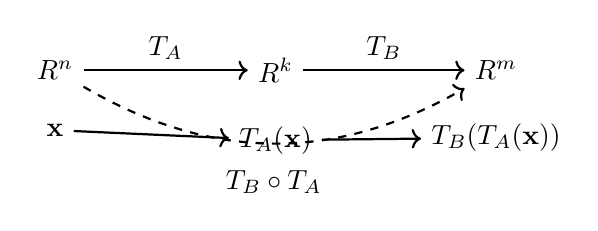
\begin{tikzpicture}[node distance=2.8cm, auto, thick]
\node (Rn) {$R^n$};
\node (Rk) [right of=Rn] {$R^k$};
\node (Rm) [right of=Rk] {$R^m$};
\node (x) [below=0.3cm of Rn] {$\mathbf{x}$};
\node (TAx) [below=0.3cm of Rk] {$T_A(\mathbf{x})$};
\node (BTAx) [below=0.3cm of Rm] {$T_B(T_A(\mathbf{x}))$};
\draw[->] (Rn) -- node[above]{$T_A$} (Rk);
\draw[->] (Rk) -- node[above]{$T_B$} (Rm);
\draw[->] (x) -- (TAx);
\draw[->] (TAx) -- (BTAx);
\draw[->, bend right=30, dashed] (Rn) to node[below=6pt]{$T_B\circ T_A$} (Rm);
\end{tikzpicture}
\end{center}

The following theorem is the key result: it shows that the composition of two matrix transformations is itself a matrix transformation, and that its standard matrix is the product of the two standard matrices (which also explains why matrix multiplication is defined as it is).

\begin{tcolorbox}[colback=red!4, colframe=red!60!black, title=Theorem 1.9.1, boxrule=0.5mm, arc=3mm]
If $T_A:R^n\to R^k$ and $T_B:R^k\to R^m$ are matrix transformations, then $T_B\circ T_A$ is also a matrix transformation and
\[
T_B\circ T_A=T_{BA} \tag{2}
\]
\end{tcolorbox}
\textbf{Proof.} We first show $T_B\circ T_A$ is linear. For vectors $\mathbf{x},\mathbf{y}\in R^n$ and scalar $k$:
\[
(T_B\circ T_A)(\mathbf{x}+\mathbf{y})=T_B(T_A(\mathbf{x}+\mathbf{y}))=T_B(T_A(\mathbf{x})+T_A(\mathbf{y}))=T_B(T_A(\mathbf{x}))+T_B(T_A(\mathbf{y}))=(T_B\circ T_A)(\mathbf{x})+(T_B\circ T_A)(\mathbf{y})
\]
\[
(T_B\circ T_A)(k\mathbf{x})=T_B(T_A(k\mathbf{x}))=T_B(kT_A(\mathbf{x}))=kT_B(T_A(\mathbf{x}))=k(T_B\circ T_A)(\mathbf{x})
\]
So $T_B\circ T_A$ is a matrix transformation; call its standard matrix $C$. Then
\[
T_C(\mathbf{x})=(T_B\circ T_A)(\mathbf{x})=T_B(T_A(\mathbf{x}))=T_B(A\mathbf{x})=B(A\mathbf{x})=(BA)\mathbf{x}=T_{BA}(\mathbf{x})
\]
By Theorem 1.8.4, $C=BA$. $\blacksquare$

\subsection*{EXAMPLE 1 | The Standard Matrix for a Composition}
Let $T_1:R^3\to R^2$ and $T_2:R^2\to R^3$ be the linear transformations
\[
T_1(x,y,z)=(x+2y,\,x+2z-y)\quad\text{and}\quad T_2(x,y)=(3x+y,\,x,\,x-2y)
\]
Find the standard matrices for $T_2\circ T_1$ and $T_1\circ T_2$.

\textbf{SOLUTION:} The standard basis vectors for $R^3$ are $\mathbf{e}_1=(1,0,0)$, $\mathbf{e}_2=(0,1,0)$, $\mathbf{e}_3=(0,0,1)$, giving
\[
T_1(\mathbf{e}_1)=(1,1),\quad T_1(\mathbf{e}_2)=(2,-1),\quad T_1(\mathbf{e}_3)=(0,2)
\implies A=\begin{bmatrix}1&2&0\\1&-1&2\end{bmatrix}
\]
The standard basis vectors for $R^2$ are $\mathbf{e}_1=(1,0)$, $\mathbf{e}_2=(0,1)$, giving
\[
T_2(\mathbf{e}_1)=(3,1,1),\quad T_2(\mathbf{e}_2)=(1,0,-2)
\implies B=\begin{bmatrix}3&1\\1&0\\1&-2\end{bmatrix}
\]
By Theorem 1.9.1, the standard matrix for $T_2\circ T_1$ is
\[
BA=\begin{bmatrix}3&1\\1&0\\1&-2\end{bmatrix}\begin{bmatrix}1&2&0\\1&-1&2\end{bmatrix}=\begin{bmatrix}4&5&2\\1&2&0\\-1&4&-4\end{bmatrix}
\]
and the standard matrix for $T_1\circ T_2$ is
\[
AB=\begin{bmatrix}1&2&0\\1&-1&2\end{bmatrix}\begin{bmatrix}3&1\\1&0\\1&-2\end{bmatrix}=\begin{bmatrix}5&1\\4&-3\end{bmatrix}
\]

\redheading{Commutativity of Matrix Transformations}

Since $AB=BA$ is not generally true, it is also not generally true that $T_{AB}=T_{BA}$, so in general
\[
T_A\circ T_B\neq T_B\circ T_A
\]
In those special cases where equality holds, we say $T_A$ and $T_B$ \textbf{commute}.

\subsection*{EXAMPLE 2 | Composition Is Not Commutative}
Let $T_A:R^2\to R^2$ be the reflection about the line $y=x$, and $T_B:R^2\to R^2$ be the orthogonal projection onto the $y$-axis. From the tables in Section 1.8, the standard matrices are
\[
A=\begin{bmatrix}0&1\\1&0\end{bmatrix},\qquad B=\begin{bmatrix}0&0\\0&1\end{bmatrix}
\]
Then
\[
AB=\begin{bmatrix}0&1\\1&0\end{bmatrix}\begin{bmatrix}0&0\\0&1\end{bmatrix}=\begin{bmatrix}0&1\\0&0\end{bmatrix},\qquad
BA=\begin{bmatrix}0&0\\0&1\end{bmatrix}\begin{bmatrix}0&1\\1&0\end{bmatrix}=\begin{bmatrix}0&0\\1&0\end{bmatrix}
\]
Since $AB\neq BA$, $T_A\circ T_B\neq T_B\circ T_A$.

\subsection*{EXAMPLE 3 | Composition of Rotations Is Commutative}
Rotating a vector through angle $\theta_1$ and then through $\theta_2$ gives the same result as the reverse order, since in both cases the net rotation angle is $\theta_1+\theta_2$. To verify algebraically, with rotation matrices $A_1=R_{\theta_1}$ and $A_2=R_{\theta_2}$:
\[
A_1A_2=\begin{bmatrix}\cos\theta_1&-\sin\theta_1\\\sin\theta_1&\cos\theta_1\end{bmatrix}\begin{bmatrix}\cos\theta_2&-\sin\theta_2\\\sin\theta_2&\cos\theta_2\end{bmatrix}=\begin{bmatrix}\cos(\theta_1+\theta_2)&-\sin(\theta_1+\theta_2)\\\sin(\theta_1+\theta_2)&\cos(\theta_1+\theta_2)\end{bmatrix}=A_2A_1
\]
using the addition formulas for sine and cosine. In rotation-matrix notation: $R_{\theta_1}R_{\theta_2}=R_{\theta_1+\theta_2}=R_{\theta_2}R_{\theta_1}$.

\subsection*{EXAMPLE 4 | Composition of Two Reflections}
Let $T_1:R^2\to R^2$ be the reflection about the $y$-axis and $T_2:R^2\to R^2$ be the reflection about the $x$-axis. Their standard matrices are $A_1=\begin{bmatrix}-1&0\\0&1\end{bmatrix}$ and $A_2=\begin{bmatrix}1&0\\0&-1\end{bmatrix}$. Both $T_1\circ T_2$ and $T_2\circ T_1$ have the same effect on any $(x,y)$:
\[
(T_1\circ T_2)(x,y)=T_1(x,-y)=(-x,-y),\qquad
(T_2\circ T_1)(x,y)=T_2(-x,y)=(-x,-y)
\]
Both compositions map $\mathbf{x}$ to $-\mathbf{x}$; this is called the \textbf{reflection about the origin}.

\begin{center}
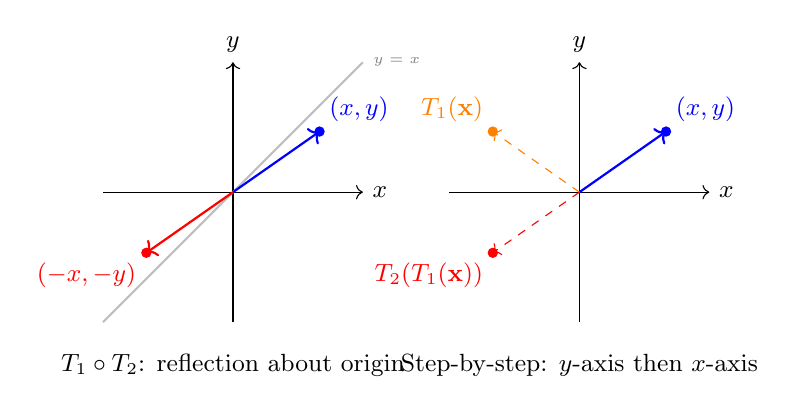
\begin{tikzpicture}[scale=1.1]
\begin{scope}[xshift=-4cm]
\draw[->] (-1.5,0)--(1.5,0) node[right]{\small $x$};
\draw[->] (0,-1.5)--(0,1.5) node[above]{\small $y$};
\draw[line width=0.8pt,gray!50] (-1.5,-1.5)--(1.5,1.5) node[right,gray]{\tiny $y=x$};
\filldraw[blue] (1,0.7) circle(1.5pt) node[above right]{\small $(x,y)$};
\draw[->,blue,thick] (0,0)--(1,0.7);
\draw[->,red,thick] (0,0)--(-1,-0.7) node[below left]{\small $(-x,-y)$};
\filldraw[red] (-1,-0.7) circle(1.5pt);
\node at (0,-2) {\small $T_1\circ T_2$: reflection about origin};
\end{scope}
\begin{scope}[xshift=0cm]
\draw[->] (-1.5,0)--(1.5,0) node[right]{\small $x$};
\draw[->] (0,-1.5)--(0,1.5) node[above]{\small $y$};
\filldraw[blue] (1,0.7) circle(1.5pt) node[above right]{\small $(x,y)$};
\draw[->,blue,thick] (0,0)--(1,0.7);
\filldraw[orange] (-1,0.7) circle(1.5pt) node[above left]{\small $T_1(\mathbf{x})$};
\draw[->,orange,dashed] (0,0)--(-1,0.7);
\filldraw[red] (-1,-0.7) circle(1.5pt) node[below left]{\small $T_2(T_1(\mathbf{x}))$};
\draw[->,red,dashed] (0,0)--(-1,-0.7);
\node at (0,-2) {\small Step-by-step: $y$-axis then $x$-axis};
\end{scope}
\end{tikzpicture}
\end{center}

For compositions of three or more transformations $T_A:R^n\to R^k$, $T_B:R^k\to R^l$, $T_C:R^l\to R^m$, the standard matrix for $T_C\circ T_B\circ T_A$ is $CBA$:
\[
T_C\circ T_B\circ T_A = T_{CBA} \tag{4}
\]

\subsection*{EXAMPLE 5 | Composition of Three Matrix Transformations}
Find the image of $\mathbf{x}=\begin{bmatrix}x\\y\end{bmatrix}$ under the composition: first rotate by $\pi/6$, then reflect about $y=x$, then project orthogonally onto the $y$-axis.

\textbf{SOLUTION:} From the tables in Section 1.8, the standard matrices are
\[
A=\begin{bmatrix}\cos(\pi/6)&-\sin(\pi/6)\\\sin(\pi/6)&\cos(\pi/6)\end{bmatrix}=\begin{bmatrix}\frac{\sqrt3}{2}&-\frac12\\\frac12&\frac{\sqrt3}{2}\end{bmatrix},\quad
B=\begin{bmatrix}0&1\\1&0\end{bmatrix},\quad
C=\begin{bmatrix}0&0\\0&1\end{bmatrix}
\]
The standard matrix for $T_C\circ T_B\circ T_A$ is
\[
CBA=\begin{bmatrix}0&0\\0&1\end{bmatrix}\begin{bmatrix}0&1\\1&0\end{bmatrix}\begin{bmatrix}\dfrac{\sqrt3}{2}&-\dfrac12\\[4pt]\dfrac12&\dfrac{\sqrt3}{2}\end{bmatrix}
=\begin{bmatrix}0&0\\0&1\end{bmatrix}\begin{bmatrix}\dfrac12&\dfrac{\sqrt3}{2}\\[4pt]\dfrac{\sqrt3}{2}&-\dfrac12\end{bmatrix}
=\begin{bmatrix}0&0\\\dfrac{\sqrt3}{2}&-\dfrac12\end{bmatrix}
\]
Thus the image is $\begin{bmatrix}0\\\frac{\sqrt3}{2}x-\frac12y\end{bmatrix}$.

\redheading{Invertibility of Matrix Operators}

If $T_A:R^n\to R^n$ is a matrix operator whose standard matrix $A$ is invertible, then $T_A$ is called \textbf{invertible}, and its \textbf{inverse} is
\[
T_A^{-1}=T_{A^{-1}} \tag{5}
\]
This is the transformation whose standard matrix is $A^{-1}$. From (5) and Theorem 1.9.1:
\[
T_A^{-1}\circ T_A=T_{A^{-1}A}=T_I \quad\text{and}\quad T_A\circ T_A^{-1}=T_{AA^{-1}}=T_I
\]
so $T_A^{-1}$ undoes the effect of $T_A$.

\subsection*{EXAMPLE 6 | Inverse of a Rotation Operator}
Let $T:R^2\to R^2$ be the counterclockwise rotation by angle $\theta$, with standard matrix $R_\theta=\begin{bmatrix}\cos\theta&-\sin\theta\\\sin\theta&\cos\theta\end{bmatrix}$.

\textbf{SOLUTION:} Geometrically, undoing a counterclockwise rotation by $\theta$ requires a clockwise rotation by $\theta$ (i.e., a rotation by $-\theta$). Indeed, from (5) and Theorem 1.4.5:
\[
R_\theta^{-1}=\begin{bmatrix}\cos\theta&\sin\theta\\-\sin\theta&\cos\theta\end{bmatrix}=\begin{bmatrix}\cos(-\theta)&-\sin(-\theta)\\\sin(-\theta)&\cos(-\theta)\end{bmatrix}=R_{-\theta}
\]

\subsection*{EXAMPLE 7 | Inverse Transformations from Linear Equations}
Consider the operator $T:R^2\to R^2$ defined by $w_1=2x_1+x_2$, $w_2=3x_1+4x_2$. Find $T^{-1}(w_1,w_2)$.

\textbf{SOLUTION:} The standard matrix is $A=\begin{bmatrix}2&1\\3&4\end{bmatrix}$, which is invertible, so
\[
A^{-1}=\begin{bmatrix}\dfrac{4}{5}&-\dfrac{1}{5}\\[6pt]-\dfrac{3}{5}&\dfrac{2}{5}\end{bmatrix}
\]
Thus the inverse transformation is
\[
T^{-1}\!\begin{bmatrix}w_1\\w_2\end{bmatrix}=A^{-1}\begin{bmatrix}w_1\\w_2\end{bmatrix}=\begin{bmatrix}\tfrac45w_1-\tfrac15w_2\\[4pt]-\tfrac35w_1+\tfrac25w_2\end{bmatrix}
\]
i.e., $T^{-1}(w_1,w_2)=\bigl(\tfrac45w_1-\tfrac15w_2,\;-\tfrac35w_1+\tfrac25w_2\bigr)$.

\noindent\textbf{Remark.} Not every matrix has an inverse; correspondingly, not every matrix transformation has an inverse. For example, the orthogonal projection operators in Section 1.8 have non-invertible standard matrices and thus have no inverse transformation.

\section*{Exercise Set 1.9}

\begin{enumerate}
\item[1.] Determine whether the operators $T_1$ and $T_2$ commute (i.e., whether $T_1\circ T_2=T_2\circ T_1$).\\
(a) $T_1:R^2\to R^2$ is the reflection about the line $y=x$, and $T_2:R^2\to R^2$ is the orthogonal projection onto the $x$-axis.\\
(b) $T_1:R^2\to R^2$ is the reflection about the $x$-axis, and $T_2:R^2\to R^2$ is the reflection about the line $y=x$.

\item[2.] Determine whether the operators commute.\\
(a) $T_1:R^2\to R^2$ is the orthogonal projection onto the $x$-axis, and $T_2:R^2\to R^2$ is the orthogonal projection onto the $y$-axis.\\
(b) $T_1:R^2\to R^2$ is the rotation through angle $\pi/4$, and $T_2:R^2\to R^2$ is the reflection about the $y$-axis.

\item[3.] $T_1:R^3\to R^3$ is the reflection about the $xy$-plane, and $T_2:R^3\to R^3$ is the orthogonal projection onto the $yz$-plane. Determine whether $T_1$ and $T_2$ commute.

\item[4.] $T_1:R^3\to R^3$ is the reflection about the $xy$-plane, and $T_2:R^3\to R^3$ is defined by $T_2(x,y,z)=(2x,3y,z)$. Determine whether $T_1$ and $T_2$ commute.

\item[5.] Let $T_A$ and $T_B$ be operators whose standard matrices are given. Find the standard matrices for $T_B\circ T_A$ and $T_A\circ T_B$.
\[
A=\begin{bmatrix}1&-2\\4&1\end{bmatrix},\qquad B=\begin{bmatrix}2&-3\\5&0\end{bmatrix}
\]

\item[7.] Find the standard matrix for the stated composition in $R^2$.\\
(a) A rotation of $90°$, followed by a reflection about the line $y=x$.\\
(b) An orthogonal projection onto the $y$-axis, followed by a $45°$ counterclockwise rotation.\\
(c) A reflection about the $x$-axis, followed by a rotation of $60°$.

\item[8.] Find the standard matrix for the stated composition in $R^2$.\\
(a) A rotation of $60°$, followed by an orthogonal projection onto the $x$-axis, followed by a reflection about the line $y=x$.\\
(b) A rotation of $15°$, followed by a rotation of $105°$, followed by a rotation of $60°$.

\item[9.] Find the standard matrix for the stated composition in $R^3$.\\
(a) A reflection about the $yz$-plane, followed by an orthogonal projection onto the $xz$-plane.\\
(b) A reflection about the $xy$-plane, followed by an orthogonal projection onto the $xy$-plane.

\item[11.] Let $T_1(x_1,x_2)=(x_1+x_2,\,x_1-x_2)$ and $T_2(x_1,x_2)=(3x_1,\,2x_1+4x_2)$.\\
(a) Find the standard matrices for $T_1$ and $T_2$.\\
(b) Find the standard matrices for $T_2\circ T_1$ and $T_1\circ T_2$.\\
(c) Use the matrices from (b) to find formulas for $T_1(T_2(x_1,x_2))$ and $T_2(T_1(x_1,x_2))$.

\item[13.] Let $T_1(x_1,x_2)=(x_1-x_2,\,2x_2-x_1,\,3x_1)$ and $T_2(x_1,x_2,x_3)=(4x_2,\,x_1+2x_2)$.\\
(a) Find the standard matrices for $T_1$ and $T_2$.\\
(b) Find the standard matrix for $T_2\circ T_1$ and $T_1\circ T_2$.\\
(c) Use the matrices from (b) to find formulas for $T_1(T_2(x_1,x_2,x_3))$ and $T_2(T_1(x_1,x_2))$.

\item[17.] Express the equations in matrix form; then use Theorem 1.5.3(c) to determine whether the operator defined by the equations is invertible.\\
(a) $w_1=8x_1+4x_2,\; w_2=2x_1+x_2$\\
(b) $w_1=-x_1+3x_2+2x_3,\; w_2=2x_1+4x_3,\; w_3=x_1+3x_2+6x_3$

\item[19.] Determine whether the operator $T:R^2\to R^2$ is invertible; if so, find the standard matrix for $T^{-1}$ and find $T^{-1}(w_1,w_2)$.\\
(a) $w_1=x_1+2x_2,\; w_2=-x_1+x_2$\\
(b) $w_1=4x_1-6x_2,\; w_2=-2x_1+3x_2$

\item[21.] Determine whether the matrix operator is invertible. If so, describe the effect of its inverse in words.\\
(a) Reflection about the $x$-axis in $R^2$.\\
(b) A $60°$ counterclockwise rotation about the origin in $R^2$.\\
(c) Orthogonal projection onto the $x$-axis in $R^2$.

\item[23.] Determine whether the operator $T_A$ is invertible. If so, compute $T_A^{-1}(\mathbf{x})$.\\
(a) $A=\begin{bmatrix}1&2\\1&1\end{bmatrix}$;\; $\mathbf{x}=\begin{bmatrix}1\\2\end{bmatrix}$\qquad
(b) $A=\begin{bmatrix}1&2&0\\1&1&1\\2&3&1\end{bmatrix}$;\; $\mathbf{x}=\begin{bmatrix}1\\2\\3\end{bmatrix}$

\item[25.] Let $T_A:R^2\to R^2$ be multiplication by
\[
A=\begin{bmatrix}0&-1\\-1&0\end{bmatrix}
\]
(a) Describe the geometric effect of applying $T_A$ to a vector $\mathbf{x}$ in $R^2$.\\
(b) Express the operator $T_A$ as a composition of two linear operators on $R^2$.

\item[27.] Prove that the matrix transformations $T_A$ and $T_B$ commute if and only if the matrices $A$ and $B$ commute.

\item[28.] Let $T_A$ and $T_B$ be matrix operators on $R^n$. Prove that $T_A\circ T_B$ is invertible if and only if both $T_A$ and $T_B$ are invertible.

\item[29.] Prove that the matrix operator $T_A$ on $R^n$ is invertible if and only if for every vector $\mathbf{b}$ in $R^n$ there exists a unique vector $\mathbf{x}$ in $R^n$ such that $T_A(\mathbf{x})=\mathbf{b}$.
\end{enumerate}

\end{document}
